\documentclass[conference]{IEEEtran}
\IEEEoverridecommandlockouts
\usepackage{cite}
\usepackage{amsmath,amssymb}
\usepackage{graphicx}
\usepackage{booktabs}
\usepackage{multirow}
\usepackage{xcolor}
\usepackage{tikz}
\usetikzlibrary{positioning,arrows.meta}
\usepackage{url}
\usepackage[hidelinks]{hyperref}

\begin{document}

\title{Predicting \emph{Toxoplasma gondii} Seropositivity from U.S.\ National Survey Data with Machine Learning: Do Biological Markers Help?}

\author{
\IEEEauthorblockN{Timothy [Surname]}
\IEEEauthorblockA{\textit{Computer Science Department} \\
\textit{School of Computing and Creative Arts} \\
Bina Nusantara University\\
Jakarta, Indonesia 11480 \\
{[email]@binus.ac.id}}
\and
\IEEEauthorblockN{Richard Hans}
\IEEEauthorblockA{\textit{Computer Science Department} \\
\textit{School of Computing and Creative Arts} \\
Bina Nusantara University\\
Jakarta, Indonesia 11480 \\
{richard.hans001@binus.ac.id}}
\and
\IEEEauthorblockN{Vickel [Surname]}
\IEEEauthorblockA{\textit{Computer Science Department} \\
\textit{School of Computing and Creative Arts} \\
Bina Nusantara University\\
Jakarta, Indonesia 11480 \\
{[email]@binus.ac.id}}
\and
\IEEEauthorblockN{Feri Setiawan}
\IEEEauthorblockA{\textit{Computer Science Department} \\
\textit{School of Computing and Creative Arts} \\
Bina Nusantara University\\
Jakarta, Indonesia 11480 \\
{feri.setiawan@binus.edu}}
\and
\IEEEauthorblockN{Nunung Nurul Qomariyah}
\IEEEauthorblockA{\textit{Computer Science Department} \\
\textit{School of Computing and Creative Arts} \\
Bina Nusantara University\\
Jakarta, Indonesia 11480 \\
{nunung.qomariyah@binus.edu}}
\and
\IEEEauthorblockN{Rizky Fajar Meirawan}
\IEEEauthorblockA{\textit{Faculty of Health Science} \\
Universitas Indonesia Maju\\
Jakarta, Indonesia 11480 \\
rizky.meirawan@gmail.com}
}

\maketitle

\begin{abstract}
Serological testing for \emph{Toxoplasma gondii} is rarely offered, so a model that estimates infection risk from survey answers could
support screening. Using the U.S.\ National Health and Nutrition Examination Survey (NHANES 2013--2014; 5,006 adults, 15.0\% seropositive),
we trained logistic regression, random forest, gradient boosting and XGBoost on demographic and lifestyle variables. The best baseline,
logistic regression, reached a cross-validated ROC-AUC of 0.722 (test 0.712). We then added 44 biological and exposure markers from 20
NHANES files: other infections, blood and environmental markers, water, diet, housing and work. The markers helped only a little: the
cross-validated ROC-AUC did not rise significantly (best 0.723), while the test ROC-AUC rose by 0.015--0.020 for logistic regression and
XGBoost. Seventeen markers remained associated with infection after adjustment for age, sex and birthplace. Pooling three NHANES cycles
(14,649 adults), modelling age flexibly, keeping the associated markers and averaging logistic regression with XGBoost gave the best
model: cross-validated ROC-AUC 0.740 ($p<0.001$) and test ROC-AUC 0.730 [0.688, 0.774]. All 5,310 NHANES variables, hyperparameter tuning
and deeper models did not go further. Prediction from NHANES is limited by the absence of direct exposure questions, not by the learners.
\end{abstract}

\begin{IEEEkeywords}
\emph{Toxoplasma gondii}, NHANES, seroprevalence, machine learning, logistic regression, random forest, XGBoost, biological markers
\end{IEEEkeywords}

\section{Introduction}
\emph{Toxoplasma gondii} infects about one third of humans \cite{montoya2004,pappas2009}. Infection is usually silent but can cause
encephalitis in people living with HIV \cite{luft1992} and congenital disease when acquired in pregnancy. Serology is the only reliable
test, and it is seldom offered where it is costly. Our earlier work trained classifiers on questionnaire data from people living with
HIV \cite{ichwan2025}. Here we use NHANES \cite{nhanes}, where a baseline model reaches a ROC-AUC of about 0.72 using age, birthplace,
education and income. These are proxies of exposure rather than exposures, which raises the question of whether biological
measurements can do better. We ask:

\begin{description}
\item[RQ1] How well do standard machine-learning models predict seropositivity from NHANES demographic and lifestyle data?
\item[RQ2] Do biological and exposure markers measured in NHANES improve these models, and which markers are associated with infection?
\item[RQ3] How far can the models be improved with more data, better use of age, ensembling and tuning, and what limits them?
\end{description}

The contributions are a comparison of four standard learners on a fixed test set, a screen of 44 markers with adjusted associations,
and an improved model with an explanation of where its limit comes from.

\begin{figure}[t]
\centering
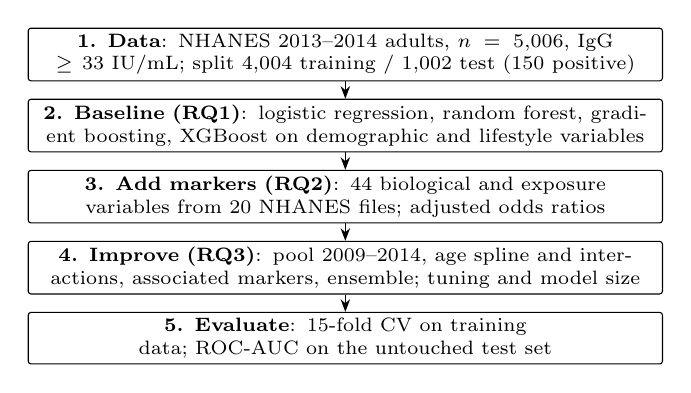
\begin{tikzpicture}[font=\scriptsize, node distance=2.2mm,
  box/.style={draw, rounded corners=1pt, align=center, inner sep=2.2pt, text width=7.9cm},
  arr/.style={-{Stealth[length=1.6mm]}, thin}]
\node[box] (a) {\textbf{1. Data}: NHANES 2013--2014 adults, $n=5{,}006$, IgG $\ge 33$ IU/mL; split 4,004 training / 1,002 test (150 positive)};
\node[box, below=of a] (b) {\textbf{2. Baseline (RQ1)}: logistic regression, random forest, gradient boosting, XGBoost on demographic and lifestyle variables};
\node[box, below=of b] (c) {\textbf{3. Add markers (RQ2)}: 44 biological and exposure variables from 20 NHANES files; adjusted odds ratios};
\node[box, below=of c] (d) {\textbf{4. Improve (RQ3)}: pool 2009--2014, age spline and interactions, associated markers, ensemble; tuning and model size};
\node[box, below=of d] (e) {\textbf{5. Evaluate}: 15-fold CV on training data; ROC-AUC on the untouched test set};
\draw[arr] (a) -- (b); \draw[arr] (b) -- (c); \draw[arr] (c) -- (d); \draw[arr] (d) -- (e);
\end{tikzpicture}
\caption{Study flow. The 1,002 test adults are used only after each model is fixed.}
\label{fig:flow}
\end{figure}

\section{Related Work}
NHANES serosurveys tracked a decline in U.S.\ seroprevalence from 1988 to 2014 and linked infection with age, foreign birth, low
education, crowding, soil-related work and region \cite{jones2001,jones2014,jones2018}. A case-control study of recently infected
patients added raw shellfish, undercooked meat, unpasteurised goat milk and kittens \cite{jones2009}. These studies report associations
but not how well individuals can be classified. Machine learning for toxoplasmosis has mostly used images; our questionnaire model for
people living with HIV \cite{ichwan2025} was trained on 78 records. Gradient-boosted trees \cite{xgboost,lightgbm} are strong on tabular
data, and overlapping cross-validation folds require corrected tests when models are compared \cite{nadeau2003}.

\section{Data and Methods}
\subsection{Cohort and Label}
Adults ($\ge 18$ years) of NHANES 2013--2014 with a Toxoplasma IgG result were included \cite{nhanes} (Table~\ref{tab:data}). A titer
$\ge 33$ IU/mL was labelled positive; equivocal results (27--33 IU/mL) were coded negative, following the CDC documentation.

\begin{table}[t]
\caption{Study Data (NHANES, Same Toxoplasma IgG Assay and Cutoff)}
\label{tab:data}
\centering
\begin{tabular}{@{}lrr@{}}
\toprule
Data & Adults & Positive (\%) \\
\midrule
NHANES 2013--2014 (main cohort) & 5,006 & 15.0 \\
\quad training set & 4,004 & 15.0 \\
\quad test set (held out) & 1,002 & 15.0 \\
NHANES 2009--2014 pooled (Sec.~III-D) & 14,649 & 17.0 \\
\bottomrule
\end{tabular}
\end{table}

\subsection{Feature Sets}
\emph{Baseline:} age, sex, race/ethnicity, years in the U.S., education, poverty--income ratio and Toxocara serostatus.
\emph{Lifestyle:} self-rated health, sleep, smoking, alcohol and the PHQ-9 depression score.
\emph{Markers:} 44 variables from 20 NHANES files: other infections (hepatitis A, with vaccination separated, E, B and C; HSV-1/2;
HIV; Toxocara IgG level), blood markers (white cells, eosinophils, lymphocytes, monocytes, haemoglobin), environmental markers (blood
lead, cadmium and mercury; cotinine), water and diet (well water, shellfish, fish, grams of each meat type eaten in a 24-hour recall),
and housing, work and poverty (crowding, renting, interview language, citizenship, farm, food-service and construction work, food
insecurity, insurance, drug use, missing teeth). Toxoplasma IgM and avidity were excluded because they measure the infection itself.
Each marker was also tested by logistic regression adjusted for age, sex and birthplace.

\subsection{Models and Evaluation}
Four standard learners were trained with fixed settings: logistic regression ($C=1$), random forest (500 trees, minimum leaf 10),
gradient boosting (300 iterations, depth 3, learning rate 0.05) and XGBoost \cite{xgboost} (300 trees, depth 3, learning rate 0.05).
Missing values were median-imputed with missing-value flags, and inputs were standardised inside each training fold (scikit-learn
\cite{sklearn}). A stratified 80/20 split (seed 42) set aside 1,002 test adults. Models were compared by 5-fold cross-validation
repeated three times on the training set, and a gain was called meaningful if the ROC-AUC rose by at least 0.01 with a corrected
repeated-CV $t$-test \cite{nadeau2003} of $p<0.05$. Each final model was scored once on the test set, with a 1,000-sample bootstrap
interval and a threshold chosen on training data (Youden's $J$).

\subsection{Improving the Model}
Five steps were added one at a time: (1) the 2009--2010 and 2011--2012 cycles, which used the same assay and cutoff (13,647 training
adults; the test set is unchanged); (2) all baseline and lifestyle variables with age as a spline; (3) age interactions with
birthplace, education and income; (4) the markers that stayed associated in the training data; and (5) averaging logistic regression
with XGBoost. We also trained on all 5,310 person-level NHANES 2013--2014 variables, ran 60 Optuna \cite{optuna} trials each for
XGBoost and LightGBM \cite{lightgbm}, and grew XGBoost from depth 2 with 300 trees to depth 10 with 5,000 trees.

\section{Results and Discussion}
\subsection{RQ1: Baseline Models}
On the baseline variables, logistic regression performed best, with a cross-validated ROC-AUC of 0.722 and a test ROC-AUC of 0.712
(Table~\ref{tab:models}, Fig.~\ref{fig:models}). Random forest (0.716), XGBoost (0.715) and gradient boosting (0.711) were close, and none
was significantly better than logistic regression. Adding the lifestyle variables did not help any model. Age, race/ethnicity and years in
the U.S.\ carried most of the signal.

\begin{table}[t]
\caption{ROC-AUC of Four Standard Models (CV: Mean $\pm$ SD Over 15 Folds; Test: 1,002 Held-Out Adults)}
\label{tab:models}
\centering
\setlength{\tabcolsep}{3pt}
\begin{tabular}{@{}lcccccc@{}}
\toprule
& \multicolumn{2}{c}{Baseline} & \multicolumn{2}{c}{+ Lifestyle} & \multicolumn{2}{c}{+ 44 markers} \\
\cmidrule(lr){2-3}\cmidrule(lr){4-5}\cmidrule(l){6-7}
Model & CV & Test & CV & Test & CV & Test \\
\midrule
Logistic reg.     & \textbf{0.722} & 0.712 & 0.718 & 0.713 & 0.699 & \textbf{0.727} \\
Random forest     & 0.716 & 0.711 & 0.717 & 0.697 & \textbf{0.723} & 0.711 \\
Gradient boost.   & 0.711 & 0.699 & 0.704 & 0.700 & 0.705 & 0.712 \\
XGBoost           & 0.715 & 0.704 & 0.713 & 0.694 & 0.708 & 0.724 \\
\midrule
CV SD (range)     & \multicolumn{6}{c}{0.016--0.022} \\
\bottomrule
\end{tabular}
\end{table}

\begin{figure}[t]
\centering
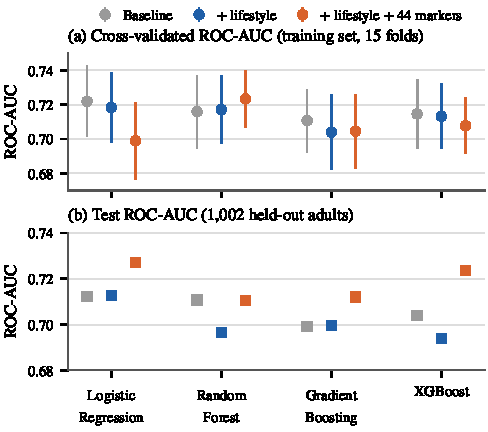
\includegraphics[width=\columnwidth]{figures/fig2_models.pdf}
\caption{ROC-AUC of the four models with baseline variables, with lifestyle variables added, and with the 44 markers added.
(a) Cross-validation (bars: $\pm1$ SD). (b) Held-out test set.}
\label{fig:models}
\end{figure}

\subsection{RQ2: Do Biological Markers Help?}
Only a little. With all 44 markers, the cross-validated ROC-AUC rose slightly for random forest (0.717 to 0.723) and fell for logistic
regression (0.718 to 0.699), which over-fits the many weak inputs; no change met the significance criterion. On the test set, the markers
raised logistic regression from 0.712 to 0.727 and XGBoost from 0.704 to 0.724 (Fig.~\ref{fig:roc}), gains within the test-set
uncertainty of about $\pm0.045$.

Seventeen of the 44 markers stayed associated with infection after adjustment (Fig.~\ref{fig:or}). The strongest were a Spanish-language
interview (OR 2.83), no health insurance (1.88), HSV-2 (1.80), non-citizenship (1.61), HSV-1 (1.46), the Toxocara IgG level (1.39 per SD) and
construction or soil work (1.30). Missing teeth, crowding, household size, blood lead and food insecurity had odds ratios of 1.17--1.20 per
SD. Shellfish (0.79) and blood mercury (0.82 per SD) were inversely associated, consistent with a fish-eating, higher-income diet. Most
markers carry the same migration and poverty signal as age and birthplace, which explains why they are associated with infection but add
little to prediction.

\begin{figure}[t]
\centering
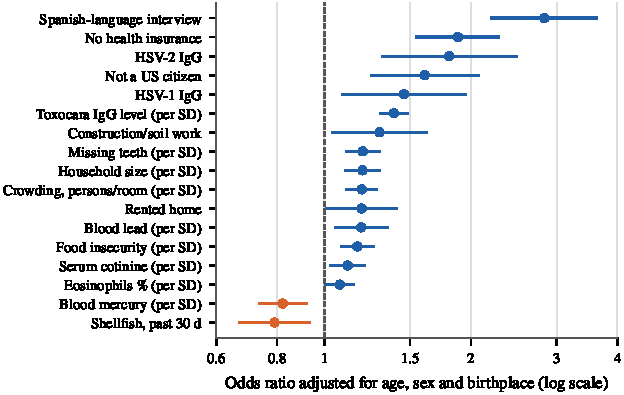
\includegraphics[width=\columnwidth]{figures/fig3_adjusted_or.pdf}
\caption{The 17 of 44 NHANES markers associated with seropositivity after adjustment for age, sex and birthplace (95\% Wald intervals).}
\label{fig:or}
\end{figure}

\begin{figure}[t]
\centering
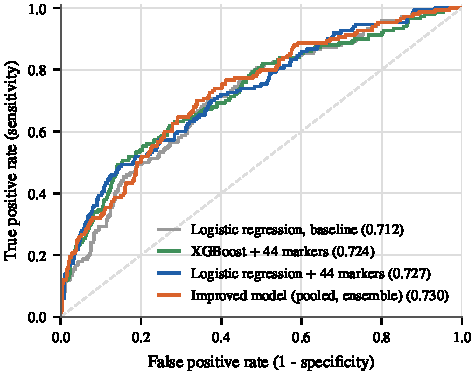
\includegraphics[width=\columnwidth]{figures/fig4_roc.pdf}
\caption{ROC curves on the 1,002 held-out adults (ROC-AUC in brackets). The improved model is described in Sec.~IV-C.}
\label{fig:roc}
\end{figure}

\subsection{RQ3: How Far Can the Models Be Improved?}
Adding the 2009--2012 cycles alone did not raise the test score (Fig.~\ref{fig:steps}a, step 1). Age terms and interactions helped
slightly, and the associated markers with a logistic regression--XGBoost average gave the best model: a cross-validated ROC-AUC of
0.740 (corrected $p=0.0002$ against step 0) and a test ROC-AUC of 0.730 [0.688, 0.774] (Table~\ref{tab:steps}). The paired bootstrap gain
over the baseline was $+0.017$ [0.000, 0.034]. At the threshold chosen on training data, the model found 70.7\% of positives with a
specificity of 64.4\% (balanced accuracy 67.6\%, against 65.8\% for the baseline). Plain accuracy is not informative here: at a
threshold of 0.5 it was 86.1\%, against 85.0\% for predicting everyone negative.

\begin{table}[t]
\caption{Improving the Model (ROC-AUC; CV on 2013--2014 Adults, Test on the 1,002 Held-Out Adults)}
\label{tab:steps}
\centering
\begin{tabular}{@{}lcc@{}}
\toprule
Model & CV & Test \\
\midrule
0 Baseline logistic regression & 0.723 & 0.713 \\
1 + 2009--2012 training data & 0.727 & 0.712 \\
2 + lifestyle, age spline & 0.726 & 0.713 \\
3 + age interactions & 0.730 & 0.714 \\
4 + associated markers & 0.735 & \textbf{0.733} \\
5 + XGBoost ensemble (final) & \textbf{0.740} & 0.730 \\
\midrule
All 5,310 NHANES variables, XGBoost & 0.721 & -- \\
Optuna-tuned XGBoost / LightGBM & 0.740 / 0.741 & 0.719 / 0.724 \\
\bottomrule
\end{tabular}
\end{table}

\begin{figure}[t]
\centering
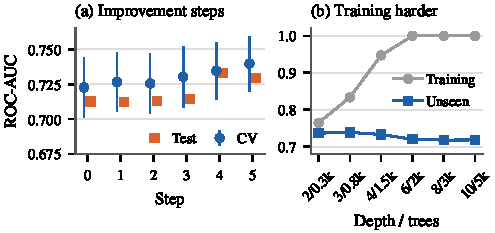
\includegraphics[width=\columnwidth]{figures/fig5_steps.pdf}
\caption{(a) Improvement steps of Table~\ref{tab:steps} (bars: $\pm1$ SD over 15 folds). (b) Training and unseen ROC-AUC as XGBoost
grows (depth / number of trees).}
\label{fig:steps}
\end{figure}

Beyond this point the models stopped improving. All 5,310 person-level NHANES variables reached 0.721, and the most used were again
interview language, age and birthplace. Tuning gave 0.740--0.741 in cross-validation but no better test score. Larger XGBoost models
memorised the training data (training ROC-AUC 0.76 $\rightarrow$ 1.00) while the score on unseen adults fell from 0.739 to 0.718
(Fig.~\ref{fig:steps}b). The limit is therefore information, not the learner: NHANES 2009--2014 asks nothing about contact with cats,
undercooked meat or soil, and IgG records infection acquired over a lifetime. Cohorts that asked these questions directly, in settings
where the exposures are common, have reached ROC-AUCs above 0.80 \cite{polanunu2021,wang2022}.

\section{Limitations and Future Work}
The data are cross-sectional and unweighted, so the models describe the NHANES sample rather than the U.S.\ population. IgG persists for
life, so present-day markers describe the person now rather than at the time of infection. Results rest on one held-out test set of 150
positives, and test-set differences below about 0.045 are within noise. Future work should add direct exposure questions (contact with
cats, undercooked meat, soil and untreated water) and validate a short questionnaire in a new cohort, including the HIV population that
motivated our earlier work.

\section{Conclusion}
Standard machine-learning models predict \emph{T.\ gondii} seropositivity from NHANES with a ROC-AUC of about 0.72, with logistic
regression as good as tree ensembles (RQ1). Adding 44 biological and exposure markers helps only a little, although 17 markers are
associated with infection (RQ2). Pooling survey cycles, modelling age flexibly and ensembling raise the score to 0.740 in cross-validation
and 0.730 on the test set, which is the practical limit for this data (RQ3). Code and derived data are available at
\url{https://github.com/Timotimanuel12/toxoplasma-research}.

\begin{thebibliography}{00}
\bibitem{montoya2004} J. G. Montoya and O. Liesenfeld, ``Toxoplasmosis,'' \emph{Lancet}, vol. 363, no. 9425, pp. 1965--1976, 2004.
\bibitem{pappas2009} G. Pappas, N. Roussos, and M. E. Falagas, ``Toxoplasmosis snapshots: Global status of \emph{Toxoplasma gondii} seroprevalence and implications for pregnancy and congenital toxoplasmosis,'' \emph{Int. J. Parasitol.}, vol. 39, no. 12, pp. 1385--1394, 2009.
\bibitem{luft1992} B. J. Luft and J. S. Remington, ``Toxoplasmic encephalitis in AIDS,'' \emph{Clin. Infect. Dis.}, vol. 15, no. 2, pp. 211--222, 1992.
\bibitem{ichwan2025} W. W. Ichwan, P. A. Tandra, N. N. Qomariyah, R. F. Meirawan, and F. Setiawan, ``Machine learning-based prediction of seropositive \emph{Toxoplasma gondii} from lifestyle factors,'' manuscript, Bina Nusantara Univ., Jakarta, Indonesia.
\bibitem{nhanes} Centers for Disease Control and Prevention, National Center for Health Statistics, ``National Health and Nutrition Examination Survey data, 2009--2014,'' Hyattsville, MD, USA. [Online]. Available: \url{https://wwwn.cdc.gov/nchs/nhanes/}
\bibitem{jones2001} J. L. Jones, D. Kruszon-Moran, M. Wilson, G. McQuillan, T. Navin, and J. B. McAuley, ``\emph{Toxoplasma gondii} infection in the United States: Seroprevalence and risk factors,'' \emph{Am. J. Epidemiol.}, vol. 154, no. 4, pp. 357--365, 2001.
\bibitem{jones2014} J. L. Jones, D. Kruszon-Moran, H. N. Rivera, C. Price, and P. P. Wilkins, ``\emph{Toxoplasma gondii} seroprevalence in the United States 2009--2010 and comparison with the past two decades,'' \emph{Am. J. Trop. Med. Hyg.}, vol. 90, no. 6, pp. 1135--1139, 2014.
\bibitem{jones2018} J. L. Jones \emph{et al.}, ``\emph{Toxoplasma gondii} infection in the United States, 2011--2014,'' \emph{Am. J. Trop. Med. Hyg.}, vol. 98, no. 2, pp. 551--557, 2018.
\bibitem{jones2009} J. L. Jones, V. Dargelas, J. Roberts, C. Press, J. S. Remington, and J. G. Montoya, ``Risk factors for \emph{Toxoplasma gondii} infection in the United States,'' \emph{Clin. Infect. Dis.}, vol. 49, no. 6, pp. 878--884, 2009.
\bibitem{nadeau2003} C. Nadeau and Y. Bengio, ``Inference for the generalization error,'' \emph{Mach. Learn.}, vol. 52, no. 3, pp. 239--281, 2003.
\bibitem{sklearn} F. Pedregosa \emph{et al.}, ``Scikit-learn: Machine learning in Python,'' \emph{J. Mach. Learn. Res.}, vol. 12, pp. 2825--2830, 2011.
\bibitem{xgboost} T. Chen and C. Guestrin, ``XGBoost: A scalable tree boosting system,'' in \emph{Proc. 22nd ACM SIGKDD Int. Conf. Knowl. Discov. Data Min.}, 2016, pp. 785--794.
\bibitem{lightgbm} G. Ke \emph{et al.}, ``LightGBM: A highly efficient gradient boosting decision tree,'' in \emph{Adv. Neural Inf. Process. Syst. (NeurIPS)}, 2017, pp. 3146--3154.
\bibitem{optuna} T. Akiba, S. Sano, T. Yanase, T. Ohta, and M. Koyama, ``Optuna: A next-generation hyperparameter optimization framework,'' in \emph{Proc. 25th ACM SIGKDD Int. Conf. Knowl. Discov. Data Min.}, 2019, pp. 2623--2631.
\bibitem{polanunu2021} N. F. A. Polanunu, S. Wahyuni, and F. Hamid, ``Seroprevalence and associated risk factors of \emph{Toxoplasma gondii} infection among pregnant mother in Makassar, Indonesia,'' \emph{PLoS ONE}, vol. 16, no. 6, art. e0245572, 2021.
\bibitem{wang2022} Z. Wang \emph{et al.}, ``Seroprevalence of \emph{Toxoplasma gondii} infection in women with a gynecological tumor living in eastern China,'' \emph{PeerJ}, vol. 10, art. e14569, 2022.
\end{thebibliography}

\end{document}
